% Tex! = xelatex
\documentclass[fontset=windows]{ctexbook}
%\usepackage{CJKpunct}
%\usepackage{showframe}
\usepackage{hyperref}
\usepackage{titletoc}
\usepackage{zhnumber}
\usepackage{fontawesome}
\usepackage{tikz}
\usepackage{ruby}
%\usepackage{emptypage} %不显示空白页页码
\usepackage{geometry}
\geometry{xetex,twoside,landscape,left=2cm,right=2cm,asymmetric=true,marginparwidth={0cm},marginparsep={15mm}}
%% 边注的宽度由长度\marginparwidth控制,与正文之间的水平距离由\marginparsep决定。
%% asymmetric参数控制左边距和右边距不会因翻页而互换。asymmetric=true表示不互换,以保证twoside模式下,头注边距的一致性。且为了页面上下对称,应满足 top = left - marginparwidth = right
\usepackage{indentfirst}
\usepackage{fancyhdr}
\usepackage{gezhu}
\expandafter\everywithgezhu\expandafter{\the\everywithgezhu}
  \everygezhu{\fontsize{11}{1}\selectfont \color{blue}} \setgezhuraise{-3.5pt}
  %\gezhuraggedture %%「」换为 ﹁﹂
\usepackage{marginnote}
\usepackage{endnotes}
\renewcommand{\notesname}{
\begin{flushleft}
  【尾注】
\end{flushleft}}
\makeatletter
\newskip\@endindent
\@endindent=1em
\long\def\@makeentext#1{\@setpar{\@@par\@tempdima \hsize
\advance\@tempdima-\@endindent
\parshape \@ne \@endindent \@tempdima}\par
\noindent \hbox to \z@{\hss\@theenmark\hspace{0.2em}}#1}
\renewcommand\theendnote{\myendnotestyle{\arabic{endnote}}}
\def\@makeenmark{\hbox{\textsuperscript{\@theenmark}}}%正文中脚注标签采取上标形式
\usepackage{pifont}
\newcommand\myendnotestyle[1]{\ifcase#1 \or \ding{192}\or \ding{193}\or
\ding{194}\or \ding{195}\or \ding{196}\or \ding{197}%
\or \ding{198}\or \ding{199}\or \ding{200}\or \ding{201}\else *\fi\relax}%数字单纯带圈,正常数字
\makeatother

\usepackage{subfig,graphicx}
% \usepackage{varwidth} %% 提供 varwidth 环境
\ctexset{
chapter/name = {第,回},
chapter/format = \leavevmode\kern-18pt\LARGE\itshape,
chapter/fixskip = true,
chapter/beforeskip = 0pt,
chapter/afterskip = 12pt
}
% \newcommand\chaptertitleformat[1]{%% 以标题内容为参数
% \begin{varwidth}[t]{.7\linewidth}#1\end{varwidth}}
%\newcommand\chaptertitle[1]{\leavevmode\kern-36pt\raise0.0pt\hbox{\fontsize{18pt}{30}\selectfont{#1}}\kern0.1pt}


\usepackage{color,xcolor}
%\usepackage{setspace}

\makeatletter
%endnotes%
\def\enoteheading{\section*{\notesname
  \@mkboth{\MakeUppercase{\notesname}}{\MakeUppercase{\notesname}}}%
  \mbox{}\par\vskip-2.3\baselineskip\noindent\rule{.5\textwidth}{0.4pt}\par\vskip\baselineskip}
\makeatletter


\makeatletter 
% 删除宏包marginnote中的margintest命令在twoside模式下奇数偶数页的边注位置判断
\renewcommand*{\@mn@margintest}{%
  \expandafter\ifx\csname @mn@thispage\endcsname\@empty
    \gdef\@mn@atthispage{1}%
  \else\expandafter\ifnum \@mn@thispage=\value{mn@abspage}%
      \begingroup
        \@tempcnta\@mn@atthispage\advance\@tempcnta by \@ne
        \xdef\@mn@atthispage{\the\@tempcnta}%
      \endgroup
    \else
      \gdef\@mn@atthispage{1}%
    \fi
  \fi
  \xdef\@mn@thispage{\themn@abspage}%
  \let\@mn@currpage\relax
  \let\@mn@currxpos\relax
  \mn@savepos
  \protected@write\@auxout{\let\themn@abspage\relax}{%
    \string\newmarginnote{note.\@mn@thispage.\@mn@atthispage}{%
      {\themn@abspage}{\noexpand\number\mn@lastxpos sp}}%
  }%
  \expandafter\ifx\csname mn@note.\@mn@thispage.\@mn@atthispage\endcsname\relax
    \if@twoside
      \if@mn@verbose
        \PackageInfo{marginnote}{Suggest that margin
          note \@mn@thispage.\@mn@atthispage\space will be on\MessageBreak
          absolute page \themn@abspage.\MessageBreak
          This may be wrong}%
      \fi
      \ifodd\value{mn@abspage}\@tempswatrue\else\@tempswafalse\fi
    \else
      \if@mn@verbose
        \PackageInfo{marginnote}{right page because not two side mode}%
      \fi
      \@tempswatrue
    \fi
  \else
    \edef\@mn@currpage{\csname
      mn@note.\@mn@thispage.\@mn@atthispage\endcsname}%
    \edef\@mn@currxpos{\expandafter\@secondoftwo\@mn@currpage}%
    \ifx\@mn@currxpos\@empty\else
      \edef\@mn@currxpos{\the\dimexpr \@mn@currxpos -\hoffset\relax}%
      \begingroup\expandafter\expandafter\expandafter\endgroup
      \expandafter\ifx\csname pdfhorigin\endcsname\relax\else
        \begingroup\expandafter\expandafter\expandafter\endgroup
        \expandafter\ifx\csname pdfoutput\endcsname\relax
          \begingroup\expandafter\expandafter\expandafter\endgroup
          \expandafter\ifx\csname outputmode\endcsname\relax\else
            \ifnum \outputmode=1 %
              \edef\@mn@currxpos{\the\dimexpr \@mn@currxpos -\pdfhorigin
                +1in\relax}%
            \fi
          \fi
        \else
          \ifnum \pdfoutput=1 %
            \edef\@mn@currxpos{\the\dimexpr \@mn@currxpos -\pdfhorigin
              +1in\relax}%
          \fi
        \fi
      \fi
      \ifdefined\mn@pagewidth
        \@mn@if@RTL{%
          \PackageInfo{marginnote}{Margin note
            \@mn@thispage.\@mn@atthispage\space in RTL mode}%
          \edef\@mn@currxpos{%
            \the\dimexpr\mn@pagewidth-\@mn@currxpos\relax
          }%
        }{}%
      \fi
    \fi
    \edef\@mn@currpage{\expandafter\@firstoftwo\@mn@currpage}%
    \if@mn@verbose
      \PackageInfo{marginnote}{Margin note \@mn@thispage.\@mn@atthispage\space
        is on absolute page \@mn@currpage}%
    \fi
    % \if@twoside
    %   \ifodd\@mn@currpage\relax
    %     \@tempswatrue
    %     \if@twocolumn
    %       \ifdim \@mn@currxpos
    %              < \dimexpr\oddsidemargin+\columnwidth+\columnsep\relax
    %         \@tempswafalse
    %       \fi
    %     \fi
    %   \else
    %     \@tempswafalse
    %     \if@twocolumn
    %       \ifdim\@mn@currxpos>\dimexpr\evensidemargin+\columnwidth\relax
    %         \@tempswatrue
    %       \fi
    %     \fi
    %   \fi
    % \else
    %   \if@mn@verbose
    %     \PackageInfo{marginnote}{right page because not two side mode}%
    %   \fi
    %   \@tempswatrue
    %   \if@twocolumn
    %     \ifdim \@mn@currxpos
    %            < \dimexpr\oddsidemargin+\columnwidth+\columnsep\relax
    %       \@tempswafalse
    %     \fi
    %   \fi
    % \fi
  \fi
}
\renewcommand{\footnotesize}{\normalsize}
\makeatletter

\makeatletter
% 设置宏包fancyhdr中的fancyplain的页眉分割线宽度为0pt(即不显示分割线)
\def\headrulewidth{0pt}%
\makeatletter

\let\oldmarginnote\marginnote
% \renewcommand\marginpar[1]{\-\oldmarginpar[\raggedleft\footnotesize #1]%
% {\raggedright\color{red}\footnotesize #1}} % 
% \marginparsep = 10pt %与正文间隔10pt
\renewcommand\marginnote[1]{\-\oldmarginnote[\raggedright\color{red}\footnotesize #1]%
{\raggedright\color{red}\footnotesize #1}} % 注释文字用红色footnote 大小

%\renewcommand{\headrulewidth}{0pt}
%\renewcommand{\chaptermark}[1]{\markright{#1}}

\renewcommand{\rightmark}{\@title}

\fancypagestyle{fancyplain}{
\fancyhf{}
<<<<<<< HEAD
\fancyhead[EL]{\leavevmode\kern18em\raise0.0pt\hbox{\fontsize{10pt}{9}\selectfont{前言}}\kern.1pt}
\fancyhead[ER]{\thepage}
\fancyfoot[OL]{{~~~~~~~~~~~~~~~~~~~~~~~~~~~~~~~~~~~~~~~~~~~~~~~~~~}\rightmark}
\fancyfoot[OR]{\thepage}
}

\fancypagestyle{fancyplain2}{
\fancyhf{}
\fancyhead[EL]{\leavevmode\kern18em\raise0.0pt\hbox{\fontsize{10pt}{9}\selectfont{后记}}\kern.1pt}
=======
%\fancyhead[EL]{{~~~~~~~~~~~~~~~~~~~~~~~~~~~~~~~~~~~~~~~~~~~~~~~~~~}前言}
\fancyhead[EL]{\leavevmode\kern18em\raise0.0pt\hbox{\fontsize{10pt}{9}\selectfont{前言}}\kern.1pt}
>>>>>>> badd52c2c2ea7b67625767fc179daf2bbcc3e9c7
\fancyhead[ER]{\thepage}
\fancyfoot[OL]{{~~~~~~~~~~~~~~~~~~~~~~~~~~~~~~~~~~~~~~~~~~~~~~~~~~}\rightmark}
\fancyfoot[OR]{\thepage}
}
%\newskip\sepskip


\fancypagestyle{maintext}{
\fancyhf{}
\fancyhead[EL]{{~~~~~~~~~~~~~~~~~~~~~~~~~~~~~~~~~~~~~~~~~~~~~~~~~~}\leftmark}
\fancyhead[ER]{\thepage}
\fancyfoot[OL]{{~}\rightmark}
\fancyfoot[OC]{{~~~~~~~~~~~~~~~~~~~~~~~~~~~~~~~~~~~~~~~~~~~~~~~~~~~~~~~~~~~~~~~~~~~~~~~~~~~~~~~~~~~~~~~~~~~~~~}\thepage}
}

\fancypagestyle{fancy}{
\fancyhf{}
\fancyhead[EL]{{~~~~~~~~~~~~~~~~~~~~~~~~~~~~~~~~~~~~~~~~~~~~~~~~~~}\leftmark}
\fancyhead[ER]{\thepage}
\fancyfoot[OL]{{~~~~~~~~~~~~~~~~~~~~~~~~~~~~~~~~~~~~~~~~~~~~~~~~~~}\rightmark}
\fancyfoot[OR]{\thepage}
}

\fancypagestyle{plain}{}

\defaultCJKfontfeatures{RawFeature={vertical:+vert:+vhal}}
\AtBeginShipout{%
  \global\setbox\AtBeginShipoutBox\vbox{%
    \special{pdf: put @thispage <</Rotate 90>>}%
    \box\AtBeginShipoutBox
  }%

}%

%\setCJKmainfont[FallBack=SimSun-ExtB]{[HaranoAjiMincho-Regular.otf]} %在ctex中 [AutoFallback = true]属性不可用。
\setCJKmainfont{SimSun} [BoldFont = SimHei , ItalicFont = KaiTi]
\xeCJKEditPunctStyle{banjiao}{optimize-kerning=false}
\newcommand*\CJKmovesymbol[1]{\raise.32em\hbox{#1}}
\newcommand*\CJKmovepunctsymbol[1]{\raise.6em\hb@xt@\z@{\hss#1}}
\newcommand*\CJKnopunctsymbol[1]{\setbox0=\hb@xt@\z@{\hss#1}\null} 
\newcommand*\CJKmove{
  
  \xeCJKnobreakbetweenpuncts
  \let\CJKsymbol\CJKmovesymbol
  \let\CJKpunctsymbol\CJKsymbol
  } %修正baseline
\AtBeginDocument{\CJKmove \sloppy}



\pagenumbering{chinese}
%\dottedcontents{chapter}[0em]{\normalsize}{4.0em}{6pt}
\titlecontents{chapter}[1cm]{\fontsize{14pt}%
{\baselineskip}\selectfont}{\hspace*{3em}\contentslabel{4em}\ }%
{}{\titlerule*[0.5pc]%
{$\cdot$}\contentspage\hspace*{1cm}}%
%titletoc宏包,它与titlesec宏包的文档写在同一个pdf文件中。

%\dottecontents{section}[left]{above-code}{label-width}{leader-width}
%\titlecontents{section}[left]{above-code}{numbered-entry-format}{numberless-entry-format}{filler-page-format}[below-code]

%各参数的含义如下所示:
%section:目录对象,可以填 chapter 、section,或者figure、table。
%left:目录对象左侧到左页边区的距离,一般必选。
%above-code:格式调整命令,可以包含垂直对象,也可以用\contentslabel,即指定本级别目录标签箱子的宽度。
%label-width:标签宽。
%leader-width:填充符号宽,默认的填充符号是圆点。
%numbered-entry-format:如果有标签,表示在目录文本前输入的格式。
%numberless-entry-format:没有标签时输入的格式。
%filler-page-format:填充格式,一般借助titlesec中的\titlerule*[width]{text}命令。
%below-code:在entry之后输入的格式,比如垂直空距。

\setlength{\parindent}{0pt} 
\setlength{\headheight}{15.7301pt}
\linespread{.9} %ctex定义的行距倍数
\setlength{\parskip}{0pt}

\title{脂硯齋重評石頭記}
\author{清\quad 曹雪芹}
\date{}
%\authorfn{庚辰本}

%%%%%%	自定義的公式 示例

\newcommand\sampleEq{%
  \left(\int_0^\infty \frac{\sin x}{\sqrt{x}}dx\right)^2
  = \sum_{k=0}^\infty \frac{(2k)!}{2^{2k}(k!)^2} \frac{1}{2k+1}
  = \prod_{k=1}^\infty \frac{4k^2}{4k^2-1}
  \neq \frac{\pi}{2015}}

%%%%%%	自定義的公式 示例(結束)
\usepackage[pages=some, scale=1,,angle=90]{background}

%\usepackage{ifthen}
%\AddEverypageHook{%
% \ifthenelse{\isodd{\value{page}}}%
% {
  \backgroundsetup{
  %angle=90,
  %position={0,0},
  contents={%
  
\begin{tikzpicture}[color={red}, remember picture, overlay,opacity=1]
    \draw[-,line width=4pt] (-7.175,6.9)--(8.475,6.9);%画外框
    \draw[-,line width=4pt] (-7.175,-12.3)--(8.475,-12.3);
    \draw[-,line width=4pt] (-7.1,6.83)--(-7.1,-12.23);
    \draw[-,line width=4pt] (8.4,6.83)--(8.4,-12.23);
    %
    \draw[-,line width=1pt] (-6.9,6.7)--(8.2,6.7);%画内框
    \draw[-,line width=1pt] (-6.9,-12.1)--(8.2,-12.1);
    \draw[-,line width=1pt] (-6.9,6.7)--(-6.9,-12.1);
    \draw[-,line width=1pt] (8.2,6.7)--(8.2,-12.1);
    %
    \draw[-,line width=1pt] (-5.73846153846154,6.7)--(-5.73846153846154,-12.1);
    \draw[-,line width=1pt] (-4.57692307692308,6.7)--(-4.57692307692308,-12.1);
    \draw[-,line width=1pt] (-3.41538461538462,6.7)--(-3.41538461538462,-12.1);
    \draw[-,line width=1pt] (-2.25384615384616,6.7)--(-2.25384615384616,-12.1);
    \draw[-,line width=1pt] (-1.09230769230769,6.7)--(-1.09230769230769,-12.1);
    \draw[-,line width=1pt] (0.0692307692307672,6.7)--(0.0692307692307672,-12.1);
    \draw[-,line width=1pt] (1.23076923076923,6.7)--(1.23076923076923,-12.1);
    \draw[-,line width=1pt] (2.39230769230769,6.7)--(2.39230769230769,-12.1);
    \draw[-,line width=1pt] (3.55384615384615,6.7)--(3.55384615384615,-12.1);
    \draw[-,line width=1pt] (4.71538461538461,6.7)--(4.71538461538461,-12.1);
    \draw[-,line width=1pt] (5.87692307692307,6.7)--(5.87692307692307,-12.1);
    \draw[-,line width=1pt] (7.03846153846153,6.7)--(7.03846153846153,-12.1);          
  \end{tikzpicture}
  }
}%
%}
% {
%   \backgroundsetup{
%   %angle=90,
%   %position={0,0},
%   contents={%
%   \begin{tikzpicture}[color={red}, remember picture, overlay]
%     \draw[-,line width=4pt] (-7.175,6.9)--(8.475,6.9);%画外框
%     \draw[-,line width=4pt] (-7.175,-12.3)--(8.475,-12.3);
%     \draw[-,line width=4pt] (-7.1,6.83)--(-7.1,-12.23);
%     \draw[-,line width=4pt] (8.4,6.83)--(8.4,-12.23);
%     %
%     \draw[-,line width=1pt] (-6.9,6.7)--(8.2,6.7);%画内框
%     \draw[-,line width=1pt] (-6.9,-12.1)--(8.2,-12.1);
%     \draw[-,line width=1pt] (-6.9,6.7)--(-6.9,-12.1);
%     \draw[-,line width=1pt] (8.2,6.7)--(8.2,-12.1);
%     %
%     \draw[-,line width=1pt] (-5.73846153846154,6.7)--(-5.73846153846154,-12.1);
%     \draw[-,line width=1pt] (-4.57692307692308,6.7)--(-4.57692307692308,-12.1);
%     \draw[-,line width=1pt] (-3.41538461538462,6.7)--(-3.41538461538462,-12.1);
%     \draw[-,line width=1pt] (-2.25384615384616,6.7)--(-2.25384615384616,-12.1);
%     \draw[-,line width=1pt] (-1.09230769230769,6.7)--(-1.09230769230769,-12.1);
%     \draw[-,line width=1pt] (0.0692307692307672,6.7)--(0.0692307692307672,-12.1);
%     \draw[-,line width=1pt] (1.23076923076923,6.7)--(1.23076923076923,-12.1);
%     \draw[-,line width=1pt] (2.39230769230769,6.7)--(2.39230769230769,-12.1);
%     \draw[-,line width=1pt] (3.55384615384615,6.7)--(3.55384615384615,-12.1);
%     \draw[-,line width=1pt] (4.71538461538461,6.7)--(4.71538461538461,-12.1);
%     \draw[-,line width=1pt] (5.87692307692307,6.7)--(5.87692307692307,-12.1);
%     \draw[-,line width=1pt] (7.03846153846153,6.7)--(7.03846153846153,-12.1);          
%   \end{tikzpicture}
%   }
%   }%
% }
  %\BgMaterial
  %\BgThispage
 %}

\begin{document}
\begin{titlepage}
  \pagestyle{empty} %封面不显示页码和页眉页脚
  \vspace*{10mm}
  \noindent{\Huge \@title}
  \vfill
  \begin{flushright}
    {\Large \@author}
  \end{flushright}
\end{titlepage}

\pagestyle{plain}
\setcounter{page}{1}
\fontsize{18}{30}\selectfont
%\newpage\NoBgThispage
\tableofcontents

%\clearpage
\pagestyle{fancyplain}
\setcounter{page}{1}
\begin{withgezhu}
  \chapter*{前言}

\par\noindent
% \marginnote{\color{cyan}%
% \zhdigits{12345}\zhdigits{67890}
% \zhdigits{12345}\zhdigits{67890}
% \zhdigits{12345}\zhdigits{67890}
% \zhdigits{12345}\zhdigits{67890}
% \zhdigits{12345}\zhdigits{67890}
% % 頭注字號{9.13}\rensuji{pt}\\\rensuji{@}11.869\rensuji{pt},
% % 行十字。 
% }
\zhdigits{12345}\zhdigits{67890}
\zhdigits{12345}\zhdigits{67890}
\zhdigits{12345}\zhdigits{67890}
\zhdigits{12345}\zhdigits{67890}
\zhdigits{12345}\zhdigits{67890}
\zhdigits{12345}\zhdigits{67890}
\zhdigits{12345}\zhdigits{67890}
\zhdigits{12345}\zhdigits{67890}
\zhdigits{12345}\zhdigits{67890}
\zhdigits{12345}\zhdigits{67890}
\zhdigits{12345}\zhdigits{67890}
\zhdigits{12345}\zhdigits{67890}
\zhdigits{12345}\zhdigits{67890}
\zhdigits{12345}\zhdigits{67890}
\zhdigits{12345}\zhdigits{67890}
\zhdigits{12345}\zhdigits{67890}
\zhdigits{12345}\zhdigits{67890}
\zhdigits{12345}\zhdigits{67890}
\zhdigits{12345}\zhdigits{67890}
\zhdigits{12345}\zhdigits{67890}
\zhdigits{12345}\zhdigits{67890}
\zhdigits{12345}\zhdigits{67890}
\zhdigits{12345}\zhdigits{67890}
\zhdigits{12345}\zhdigits{67890}
\zhdigits{12345}\zhdigits{67890}
% \hspace{1zw}使用\verb+\LARGE+命令調用\dash\\
% 正文字號{15.521}\rensuji{pt}\rensuji{@}{27.39}\rensuji{pt},
% 一行\rensuji{31}字。正文與割注換算關係為:

\begin{center}
\noindent
一個正文字 = 1.67 割注字\footnote{脚注測試:序號為一}
\\%
\setcounter{footnote}{98}
一個正文字 = 2 行間注字\footnote{脚注測試:序號最大為九十九}
\endnote{需使用以下命令為行間注設置字號,使之恰好為正文字號的一半。}
% {\ttfamily $\backslash$rubyfontsetup\{$\backslash$mgfamily
% $\backslash$fontsize\{8.5pt\}\{10\}$\backslash$selectfont\} }\\[2mm]
% 另一個方法,自動模式:不設置字號,只設置字體風格,默認振假名為正文字號的一半。如:\\ \hspace{2zw}
% {\ttfamily $\backslash$rubyfontsetup\{$\backslash$mgfamily$\backslash$selectfont\} }}
\end{center}

\gezhu{
\zhdigits{12345}\zhdigits{67890}
\zhdigits{12345}\zhdigits{67890}
\zhdigits{12345}\zhdigits{67890}
\zhdigits{12345}\zhdigits{67890}\\
\zhdigits{12345}\zhdigits{67890}
\zhdigits{12345}\zhdigits{67890}
\zhdigits{12345}\zhdigits{67890}
\zhdigits{12345}\zhdigits{67890}\\
雙行割注字號{9.13}pt\faAt{9.13}pt in real diemen
}

% \clearpage
% \par\noindent{\normalsize
% 正文 normalsize,字號{9.13}\rensuji{pt}\rensuji{@}{16.434}\rensuji{pt},
% 行\rensuji{55}字。\\
% \zhdigits{12345}\zhdigits{67890}
% \zhdigits{12345}\zhdigits{67890}
% \zhdigits{12345}\zhdigits{67890}
% \zhdigits{12345}\zhdigits{67890}
% \zhdigits{12345}\zhdigits{67890}
% \zhdigits{12345}\zhdigits{67890}}


% \par\noindent{\fontsize{11pt}{12}\selectfont
% 測試字號{10.043}\rensuji{pt}\rensuji{@}{10.043}\rensuji{pt},
% 行\rensuji{50}字。\\
% \zhdigits{12345}\zhdigits{67890}
% \zhdigits{12345}\zhdigits{67890}
% \zhdigits{12345}\zhdigits{67890}
% \zhdigits{12345}\zhdigits{67890}
% \zhdigits{12345}\zhdigits{67890}
% \zhdigits{12345}\zhdigits{67890}}

\theendnotes
\newpage

\end{withgezhu}


\newgeometry{twoside,left=8cm,right=2cm,asymmetric=true,marginparwidth={4.5cm},marginparsep={15mm}}

%\newpage
%\clearpage
\pagestyle{maintext}
\renewcommand\baselinestretch{1.1}\selectfont




\begin{withgezhu}
  \setcounter{page}{1}

  %\input{text/bodytext1.tex}
  %\newpage
  \AddEverypageHook{%此后每页都添加网格
  \BgMaterial
  }
  \setcounter{chapter}{15}
\chapter{賈元春才選鳳藻宮 秦鯨卿夭逝黃泉路}
%\reversemarginpar
%\rubyfontsetup{\fontsize{8.5pt}{10}\selectfont}  % truely 7.760 pt in real dimen.
%賈元春才選鳳藻宮 秦鯨卿夭逝黃泉路\\
{\leavevmode\kern-18pt\raise0.0pt\hbox{\fontsize{18pt}{30}\selectfont{賈璉}}\kern0.1pt}%
%raise box 是用來給挪格用的.\kern和、raise只能作用于hbox或vbox对象
此時没好意思,\marginnote{〔庚〕大觀園用省親事出題,是大関鍵事,方見大手筆行文之立意。%
\begin{flushright}
畸笏。%
\end{flushright} \par {~}\par
趙媽一問是文章家進一步門庭法則。\par
〔庚〕自政老生日,用降旨截住,賈母等進朝如此熱鬧,用秦業死岔開,只冩幾個﹁如何﹂,%
將潑天喜事交代完了,緊接黛玉回,璉、鳳閒話,以老嫗勾出省親事来。其千頭萬緒,合榫%
貫連,無一毫痕跡,如此等,是書多多,不能枚舉。想兄在青峺峰上,經煅煉後,參透重関%
至恒河沙數。如否,余曰萬不能有此機括,有此筆力,恨不得面問果否。嘆嘆!%
\begin{flushright}
丁亥春。畸笏叟。% 
\end{flushright} \par
}
只是訕笑吃酒,說﹁胡說﹂二字,﹁快盛飯来,吃碗子還要往珍大爺那邊去商議事呢。﹂%
鳳姐道:﹁可是別悞了正事。纔剛老爺叫你作什麼?﹂%
\gezhu{一段趙嫗討情閒文,却引出通部脈絡。所謂由小及大,譬如登高必自卑之意。%
細思大觀園一事,若從如何奉旨起造,又如何分派衆人,從頭細細直冩將来,幾千樣細事,%
如何能順筆一氣冩清?又將落於死板拮据之鄕,故只用璉鳳夫妻二人一問一答,上用趙嫗%
討情作引,下用蓉薔来說事作收,餘者隨筆順筆略一點染,則耀然洞徹矣。此是避難法。}%
賈璉道:\ruby{{﹁就爲{省親}。﹂}}{{{二字醒眼之極,却只如此冩来。}}}%
鳳姐忙問道:\gezhu{﹁忙﹂字最要緊,特於鳳姐口中出此字,可知事関巨要,非同淺細,是此書中正眼矣。}%
﹁省親的事竟準了不成?﹂\gezhu{問得珍重,可知是萬人意外之事。(脂硯)}%
賈璉笑道:﹁雖不十分準,也有八分準了。﹂\gezhu{如此故頓一筆,更妙!見得事関重大,非一語可了者,亦是大篇文章,抑揚頓%
挫之至。}鳳姐笑道:﹁可見當今的隆恩。歷来聽書看戲,古時從未有的。﹂\gezhu{於閨閣中作此語,直與〈擊壤〉同聲。(脂硯)}%
趙媽又接口道:%\zmark{16A8}	%	因前一頁排不下故挪至第二頁
﹁可是呢,我也老糊塗了。我聽見上下吵嚷了這些日子,什麼省親不省親,%
我也不理論他去;如今又說省親,到底是怎麼個原故?﹂賈璉道:﹁%
\ruby{{如今當今貼體萬人之心,世上至大莫如『孝』}}{{{大觀園一篇大文,千頭萬緒,%
從何處冩起,今故用賈璉夫妻問答之間,閒閒敘出,}}}\ruby{{字,想来父母児女之性,皆是一理,不是貴%
}}{{{觀者已省大半。後再用蓉、薔二人重一渲染。便省却多少贅瘤筆墨。此是避難法。}}}%
賤上分別的。當今自爲日夜侍奉太上皇、皇太后,尚不能略盡孝意,因見宮裡嬪妃才人等%
皆是入宮多年,以致抛離父母音容,豈有不思想之理?在児女思想父母,是分所應當。想%
父母在家,若只管思念児女,竟不能一見,倘因此成疾致病,甚至死亡,皆由朕躬禁錮,%
不能使其遂天倫之願,亦大傷天和之事。故啓奏太上皇、皇太后,每月逢二六日期,準其%
椒房眷屬入宮請安看視。于是太上皇、皇太后大喜,深讚當今至孝純仁,體天格物。因此%
二位老聖人又下旨意,說椒房眷屬入宮,未免有國體儀制,母女尚不能愜懷。竟大開方便%
之恩,特降諭諸椒房貴戚,除二六日入宮之恩外,凡有重宇別院之家,可以駐蹕関防之處,%
不妨啓請內廷鑾輿入其私第,庶可略盡骨肉私情、天倫中之至性。此旨一下,誰不踴躍感%
戴?現今周貴人父親已在家裡動了工了,修蓋省親別院呢。又有吳貴妃的父親吳天佑家,%
也往城外\ruby{{踏看地方}}{{{又一樣佈置。}}}去了。這豈非有八九分了?﹂%

{\leavevmode\kern-18pt\raise0.0pt\hbox{\fontsize{18pt}{30}\selectfont{賈璉}}\kern0.1pt}%
%raise box 是用來給挪格用的.\kern和、raise只能作用于hbox或vbox对象
此時没好意思,\marginnote{〔庚〕大觀園用省親事出題,是大関鍵事,方見大手筆行文之立意。%
\begin{flushright}
畸笏。%
\end{flushright} \par {~}\par
趙媽一問是文章家進一步門庭法則。\par
〔庚〕自政老生日,用降旨截住,賈母等進朝如此熱鬧,用秦業死岔開,只冩幾個﹁如何﹂,%
將潑天喜事交代完了,緊接黛玉回,璉、鳳閒話,以老嫗勾出省親事来。其千頭萬緒,合榫%
貫連,無一毫痕跡,如此等,是書多多,不能枚舉。想兄在青峺峰上,經煅煉後,參透重関%
至恒河沙數。如否,余曰萬不能有此機括,有此筆力,恨不得面問果否。嘆嘆!%
\begin{flushright}
丁亥春。畸笏叟。% 
\end{flushright} \par
}
只是訕笑吃酒,說﹁胡說﹂二字,﹁快盛飯来,吃碗子還要往珍大爺那邊去商議事呢。﹂%
鳳姐道:﹁可是別悞了正事。纔剛老爺叫你作什麼?﹂%
\gezhu{一段趙嫗討情閒文,却引出通部脈絡。所謂由小及大,譬如登高必自卑之意。%
細思大觀園一事,若從如何奉旨起造,又如何分派衆人,從頭細細直冩將来,幾千樣細事,%
如何能順筆一氣冩清?又將落於死板拮据之鄕,故只用璉鳳夫妻二人一問一答,上用趙嫗%
討情作引,下用蓉薔来說事作收,餘者隨筆順筆略一點染,則耀然洞徹矣。此是避難法。}%
賈璉道:\ruby{{﹁就爲{省親}。﹂}}{{{二字醒眼之極,却只如此冩来。}}}%
鳳姐忙問道:\gezhu{﹁忙﹂字最要緊,特於鳳姐口中出此字,可知事関巨要,非同淺細,是此書中正眼矣。}%
﹁省親的事竟準了不成?﹂\gezhu{問得珍重,可知是萬人意外之事。(脂硯)}%
賈璉笑道:﹁雖不十分準,也有八分準了。﹂\gezhu{如此故頓一筆,更妙!見得事関重大,非一語可了者,亦是大篇文章,抑揚頓%
挫之至。}鳳姐笑道:﹁可見當今的隆恩。歷来聽書看戲,古時從未有的。﹂\gezhu{於閨閣中作此語,直與〈擊壤〉同聲。(脂硯)}%
趙媽又接口道:%\zmark{16A8}	%	因前一頁排不下故挪至第二頁
﹁可是呢,我也老糊塗了。我聽見上下吵嚷了這些日子,什麼省親不省親,%
我也不理論他去;如今又說省親,到底是怎麼個原故?﹂賈璉道:﹁%
\ruby{{如今當今貼體萬人之心,世上至大莫如『孝』}}{{{大觀園一篇大文,千頭萬緒,%
從何處冩起,今故用賈璉夫妻問答之間,閒閒敘出,}}}\ruby{{字,想来父母児女之性,皆是一理,不是貴%
}}{{{觀者已省大半。後再用蓉、薔二人重一渲染。便省却多少贅瘤筆墨。此是避難法。}}}%
賤上分別的。當今自爲日夜侍奉太上皇、皇太后,尚不能略盡孝意,因見宮裡嬪妃才人等%
皆是入宮多年,以致抛離父母音容,豈有不思想之理?在児女思想父母,是分所應當。想%
父母在家,若只管思念児女,竟不能一見,倘因此成疾致病,甚至死亡,皆由朕躬禁錮,%
不能使其遂天倫之願,亦大傷天和之事。故啓奏太上皇、皇太后,每月逢二六日期,準其%
椒房眷屬入宮請安看視。于是太上皇、皇太后大喜,深讚當今至孝純仁,體天格物。因此%
二位老聖人又下旨意,說椒房眷屬入宮,未免有國體儀制,母女尚不能愜懷。竟大開方便%
之恩,特降諭諸椒房貴戚,除二六日入宮之恩外,凡有重宇別院之家,可以駐蹕関防之處,%
不妨啓請內廷鑾輿入其私第,庶可略盡骨肉私情、天倫中之至性。此旨一下,誰不踴躍感%
戴?現今周貴人父親已在家裡動了工了,修蓋省親別院呢。又有吳貴妃的父親吳天佑家,%
也往城外\ruby{{踏看地方}}{{{又一樣佈置。}}}去了。這豈非有八九分了?﹂%


  
\end{withgezhu}

\clearpage\cleardoublepage
\newpage
\pagestyle{fancyplain2}
\newgeometry{twoside,andscape,left=2cm,right=2cm,asymmetric=true,marginparwidth={0cm},marginparsep={15mm}}
\begin{withgezhu}
\chapter{畫圖測試}

\begin{minipage}[htpb]{80mm}
	%\begin{center}
    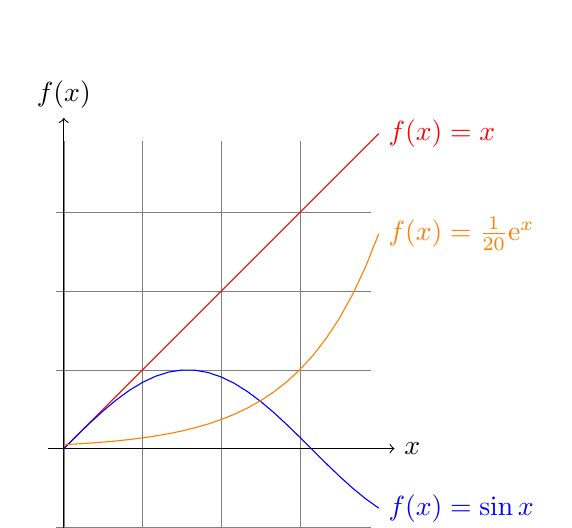
\begin{tikzpicture}[domain=0:4]
		  \draw[very thin,color=gray] (-0.1,-1.1) grid (3.9,3.9);
  		\draw[->] (-0.2,0) -- (4.2,0) node[right] {$x$};
		  \draw[->] (0,-1.2) -- (0,4.2) node[above] {$f(x)$};
		  \draw[color=red]    plot (\x,\x)             node[right] {$f(x) =x$};
  % \x r 表示弧度
		  \draw[color=blue]   plot (\x,{sin(\x r)})    node[right] {$f(x) = \sin x$};
		  \draw[color=orange] plot (\x,{0.05*exp(\x)}) node[right] {$f(x) = \frac{1}{20} \mathrm e^x$};
		\end{tikzpicture}
	%\end{center}
\end{minipage}



\begin{minipage}[htpb][80mm][t]{80mm}
	%\begin{center}
		\vspace*{60mm}
    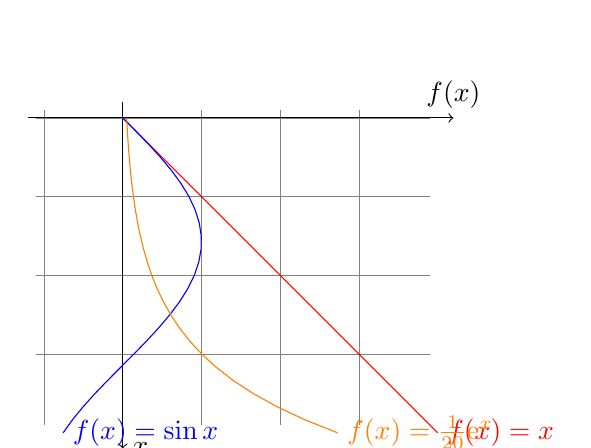
\begin{tikzpicture}[domain=0:4,scale=1,rotate=270]
		  \draw[very thin,color=gray] (-0.1,-1.1) grid (3.9,3.9);
  		\draw[->] (-0.2,0) -- (4.2,0) node[right] {$x$};
		  \draw[->] (0,-1.2) -- (0,4.2) node[above] {$f(x)$};
		  \draw[color=red]    plot (\x,\x)             node[right] {$f(x) =x$};
  % \x r 表示弧度
		  \draw[color=blue]   plot (\x,{sin(\x r)})    node[right] {$f(x) = \sin x$};
		  \draw[color=orange] plot (\x,{0.05*exp(\x)}) node[right] {$f(x) = \frac{1}{20} \mathrm e^x$};
		\end{tikzpicture}
	%\end{center}
\end{minipage}

% \chapter{公式測試}

\vskip 20 mm
\begin{minipage}[htpb]{80mm}
		\vspace*{45mm}
	%\begin{center}
			{\normalsize With normalsize 10 pt in class (truely 9.13\,pt in real dimen):
				\[ \sampleEq \]\par}

			{\Large With Large 14 pt in class (truely 12.782\,pt in real dimen):
				\[ \sampleEq \]\par}

			{\footnotesize With footnotesize 8 pt in class (truely 7.304\,pt in real dimen):
				\[ \sampleEq \]\par}
	%\end{center}
\end{minipage}

\clearpage
\begin{minipage}[htpb]{120mm}
		\vspace*{10mm}
	%\begin{center}
			{\normalsize 
				\[ \sampleEq \]\par}

			{\Large 
				\[ \sampleEq \]\par}

			{\footnotesize
				\[ \sampleEq \]\par}
	%\end{center}
\end{minipage}
\end{withgezhu}
\restoregeometry
\end{document}

